%!TEX root = ../thesis.tex
%*******************************************************************************
%****************************** MFHBO Chapter **********************************
%*******************************************************************************
\chapter{Multi-Frame Binary-Phase Holograms Batched Optimisation}
\label{chapter:Multi Frame Holograms Batched Optimisation}

\graphicspath{{Chapter_MFHBO/Figs/}}

\textit{Note: The work in this chapter has been published in Ref. \cite{Sha2024MFHBO}}\\\\

This chapter builds up on the idea of time-averaging multiple hologram frames, and proposes a technique called Multi-Frame Holograms Batched Optimisation (MFHBO), which uses the L-BFGS optimisation algorithm to simultaneously generate a batch of phase-only holograms which result in an average reconstructed image of improved fidelity and fast algorithmic convergence, both in the Fraunhofer and the Fresnel regions.

\section{Introduction}
	\cref{chapter:L-BFGS Optimisation of Phase-Only Hologram} implemented optimisation algorithms to generate single-frame holograms. This chapter proposes the novel MFHBO method which optimise a batch of multi-frame holograms for time multiplexing. Time multiplexing seeks to improve a time-averaged response by displaying different hologram sub-frames at a high refresh rate \cite{Amako1995}. Such approach can exploit the finite response time of human vision, where human eyes average out the unwanted noise while the wanted signal remains. A few time-multiplexed multi-frame holograms generation methods have been explored in the literature, including the OSPR algorithm in \cref{sec:One Step Phase Retrieval (OSPR) Algorithm} and the AD-OSPR algorithm in \cref{sec:Adaptive One-Step Phase Retrieval (AD-OSPR) Algorithm}; however, both OSPR and AD-OSPR are still subject to noise and defects in reconstruction quality. The objective of the proposed MFHBO algorithm is therefore to produce a batch of holograms having better reconstruction quality than the existing OSPR and AD-OSPR methods.


\section{Methods}
	The use of the L-BFGS algorithm for single-frame hologram optimisation has been introduced in \cref{chapter:L-BFGS Optimisation of Phase-Only Hologram}. To implement it onto multi-frame holograms generation, the argument to optimise becomes the set of holograms with $n$ sub-frames ($\{\textbf{H}_1, \textbf{H}_2, ..., \textbf{H}_n\}$), each having a resolution of $X\times Y$ pixels matching the resolution of the target image, and the objective function to minimise is therefore the difference between the average reconstruction amplitude ($\textbf{R}_{avg}=\frac{1}{n}\sum_{i=1}^n\textbf{R}_i$) and the target image ($\textbf{T}$), which is denoted as $Loss(\textbf{T}, \textbf{R}_{avg})$, where $n$ is the total number of frames, $\textbf{R}_i$'s are reconstructions from individual hologram sub-frames $\textbf{H}_i$'s for $i\in[1,n]$. To compute each $\textbf{R}_i$ from the corresponding $\textbf{H}_i$, the Fresnel diffraction formula given in \cref{eq:fresnel-diffraction} is used. As we are generating holograms for phase-only SLM's, the hologram aperture $\textbf{A}$ in \cref{eq:fresnel-diffraction} is then comprised of a uniform amplitude with phase $\textbf{H}$, giving $\textbf{A} = e^{j\textbf{H}}$, where the exponential is taken element-wise, and the replay field($\textbf{E}$)'s amplitude is the reconstruction (i.e.$\textbf{R} = |\textbf{E}|$).

	\begin{figure}[H]
		\centering
		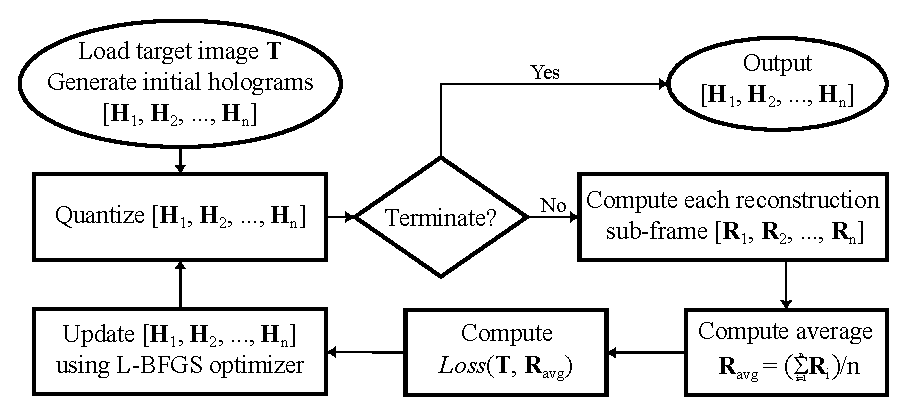
\includegraphics[width=0.9\textwidth]{MFHO_flowchart.eps}
		\caption{MFHBO flowchart}
		\label{fig:MFHO_flowchart}
	\end{figure}

	To help explain the optimisation process, a flow chart is drawn in \cref{fig:MFHO_flowchart}. As shown in the flowchart, the target image $\textbf{T}$ is first loaded, with a set of $n$ hologram sub-frames ($\{\textbf{H}_1, \textbf{H}_2, ..., \textbf{H}_n\}$) generated randomly. Then at every iteration, each hologram sub-frame $\textbf{H}_i$ is quantised to the bit-depth constraint of the SLM, and propagated to the reconstruction plane $\textbf{R}_i$, and the average of the amplitudes of all reconstructions $\textbf{R}_{avg}$ is computed and compared against the target image $\textbf{T}$ using a loss function $Loss(\textbf{T}, \textbf{R}_{avg})$, after which the search direction is computed using the L-BFGS optimiser and the hologram sub-frames are updated accordingly. Here the loss function selected is the relative entropy\cite{Kullback1951} given in \cref{eq:RE_holo}.

	% \begin{equation}
	% 	Loss(\textbf{T}, \textbf{R}_{avg}) = -\sum_{x=1}^{X} \sum_{y=1}^{Y} \textbf{T}_{(x,y)}\log\left(\frac{\textbf{R}_{avg(x,y)}}{\textbf{T}_{(x,y)}}\right)
	% 	\label{eq:RE_holo}
	% \end{equation}

	Since fast SLM's available in the lab are binary-phase devices, the quantisation step in the flowchart in \cref{fig:MFHO_flowchart} is carried out with bit-depth limit of 1, hence producing binary-phase holograms. However, the optimisation algorithm does not converge with a straight binary quantisation as integers are discrete, therefore a Sigmoid function \cite{Bacaer2011} is used for a smoother and differentiable quantisation, as defined in \cref{eq:sigmoid}. The output of the Sigmoid function is then scaled by $\pi$ so that the binary phase levels are $0$ and $\pi$.

	\begin{equation}
		\mathrm{sigmoid}(x)=\frac{1}{1+e^{-x}}
		\label{eq:sigmoid}
	\end{equation}

	And finally, when displaying the multi-frame holograms, each of the $n$ frames generated are then rounded to binary phase values and displayed on the binary phase SLM sequentially. And when the first round finished, the second round starts with the first frame again (i.e. after frame $n$, the next frame displayed is frame $1$), and such infinite loop doesn't stop until another set of holograms are uploaded.

\section{Results}

\subsection{Simulation results}
	To test the proposed MFHBO method, a target image $\textbf{T}$ as shown in \cref{fig:optim_iter_flowchart} was used. It was designed from the widely used mandrill image \cite{MANDRILL_REF} in \cref{fig:mandrill.png}. A rotational symmetry was introduced to match the rotational symmetry of the far field projection from binary phase holograms, as explained in \cref{sec:Rotational symmetries in the binary phase modulation}. It was then zero padded to a resolution of $1024px\times 1024px$ and subsequently interpolated (using the `$torch.nn.functional.interpolate$' function in the PyTorch module\cite{Paszke2019}) to a resolution of $1280px\times 1024px$ to match the resolution of the SLM in our lab. Note that the target image was zero padded to a square aspect ratio and then stretched to the non-square aspect ratio because more pixels in the horizontal axis only means higher sampling rate as part of the features of the FFT, the replay field is continuous and is not pixelated and the simulated reconstruction of $1280px\times 1024px$ resolution is the sampled result, which will be illustrated visually in \cref{fig:recon_quality_vs_num_frames} later.

	\begin{figure}[H]
		\centering
		\includegraphics[width=1.0\textwidth]{optim_iter_flowchart.pdf}
		\caption{An example iteration in the optimisation process}
		\label{fig:optim_iter_flowchart}
	\end{figure}

	To further explain the optimisation process described in \cref{fig:MFHO_flowchart}, an example iteration with $n=24$ is shown in \cref{fig:optim_iter_flowchart}. At each iteration, every hologram is quantised and propagated to the reconstruction plane, forming $\{\textbf{R}_1, \textbf{R}_2, ..., \textbf{R}_{24}\}$. The average reconstruction amplitude $\textbf{R}_{avg}$ is then compared against the target image $\textbf{T}$, using the loss function in \cref{eq:RE_holo}. The holograms $\{\textbf{H}_1, \textbf{H}_2, ..., \textbf{H}_{24}\}$ are then updated according to the search direction calculated using the L-BFGS optimiser. After setting the optimisation to terminate when the number of iterations reach $1000$, the same algorithm was run on the same target for different number of frames ($n$), the normalised mean squared error (NMSE) and the peak signal-to-noise ratio (PSNR) between the average reconstruction $\textbf{R}_{avg}$ and the target image $\textbf{T}$ were calculated at every iteration and plotted in \cref{fig:Mandrill_NMSE_vs_iter} and \cref{fig:Mandrill_PSNR_vs_iter} respectively.

	\begin{figure}[H]
		\centering
		\begin{subfigure}[t]{0.7\textwidth}
			\centering
			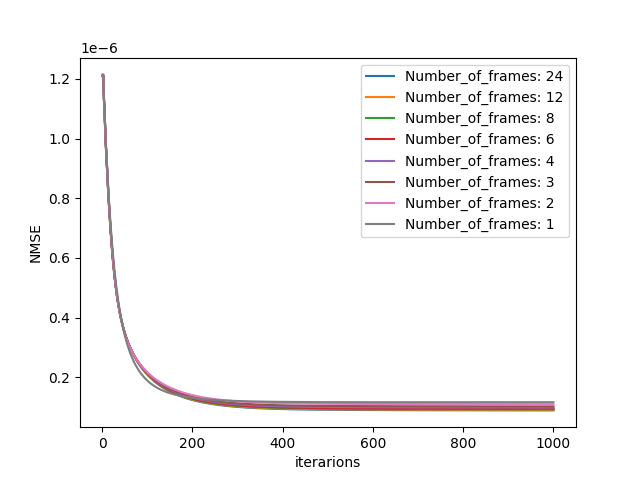
\includegraphics[width=1.0\textwidth]{Mandrill_NMSE_vs_iter.png}
			\caption{NMSE v.s. Iteration Number}
			\label{fig:Mandrill_NMSE_vs_iter}
		\end{subfigure}
		\\
		\begin{subfigure}[t]{0.7\textwidth}
			\centering
			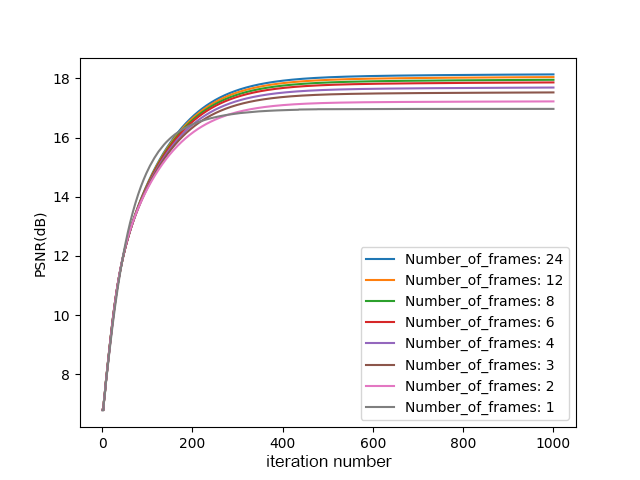
\includegraphics[width=1.0\textwidth]{Mandrill_PSNR_vs_iter.png}
			\caption{PSNR v.s. Iteration Number}
			\label{fig:Mandrill_PSNR_vs_iter}
		\end{subfigure}
		\caption{Convergence of the MFHBO algorithm on the rotationally symmetrical Mandrill target}
		\label{fig:Convergence of optimisation}
	\end{figure}

	The plots in \cref{fig:Convergence of optimisation} show that the proposed MFHBO method has achieved good convergence within 400 iterations, for the various number of frame settings $n$ in $\{1, 2, 3, 4, 6, 8, 12, 24\}$. The final NMSE values in \cref{fig:Mandrill_NMSE_vs_iter} are difficult to distinguish in the plot, therefore it will be further compared in the bar chart in \cref{fig:recon_quality_vs_num_frames}. The number of frames are chosen to be integer factors of $24$, which is determined by our experimental setup, further explained in the next subsection.


	\begin{table}[H]
	\centering
	\begin{tabular}{|c|c|c|c|c|c|}
	\hline
	\textbf{n} & \textbf{200 iterations} & \textbf{400 iterations} & \textbf{600 iterations} & \textbf{800 iterations} & \textbf{1000 iterations} \\ \hline
	1 & 1.79 & 3.59 & 5.31 & 7.00 & 8.72 \\ \hline
	2 & 2.82 & 5.59 & 8.34 & 11.11 & 13.88 \\ \hline
	3 & 3.84 & 7.67 & 11.45 & 15.21 & 19.00 \\ \hline
	4 & 4.93 & 9.83 & 14.70 & 19.58 & 24.47 \\ \hline
	6 & 6.95 & 13.87 & 20.76 & 27.58 & 34.50 \\ \hline
	8 & 8.87 & 17.67 & 26.54 & 35.60 & 44.56 \\ \hline
	12 & 12.95 & 25.79 & 38.63 & 51.47 & 64.30 \\ \hline
	24 & 51.81 & 101.43 & 151.09 & 201.08 & 251.15 \\ \hline
	\end{tabular}
	\caption{MFHBO runtime (s)}
	\label{tab:MFHBO runtime}
	\end{table}

	The programme runtime of the proposed MFHBO method has been measured on a laptop computer of model ASUS ROG Zephyrus M16 (GU603H) with a CPU of model i7-11800H and a GPU of model NVIDIA RTX3060 and the results for different combinations of number of frames and number of iterations are listed in \cref{tab:MFHBO runtime}. It can be concluded that the application of the proposed method is for pre-computed high-quality holograms, instead of real-time holographic projection.



\subsection{Optical Experiment results}

	The holographic projection system used in this experiment is the same as the one described in \cref{sec:experimental setup}, with the optical setup shown in \cref{fig:holographic_projector}. Since the SLM has a refresh rate of 1440Hz and modern computer monitors have refresh rate of at least 60Hz, the maximum number of frames was chosen to be $1440/60=24$, so that each set of 24 frames will take a total of $1/60$ seconds to display, therefore giving an equivalent refresh rate of 60Hz. Then the integer factors of 24 were chosen so that the equivalent refresh rate becomes integer multiples of 60Hz. The number of frames starts from 1 to help illustrate how the increase in number of frames positively affect the reconstruction quality.

	\begin{figure}[H]
		\centering
		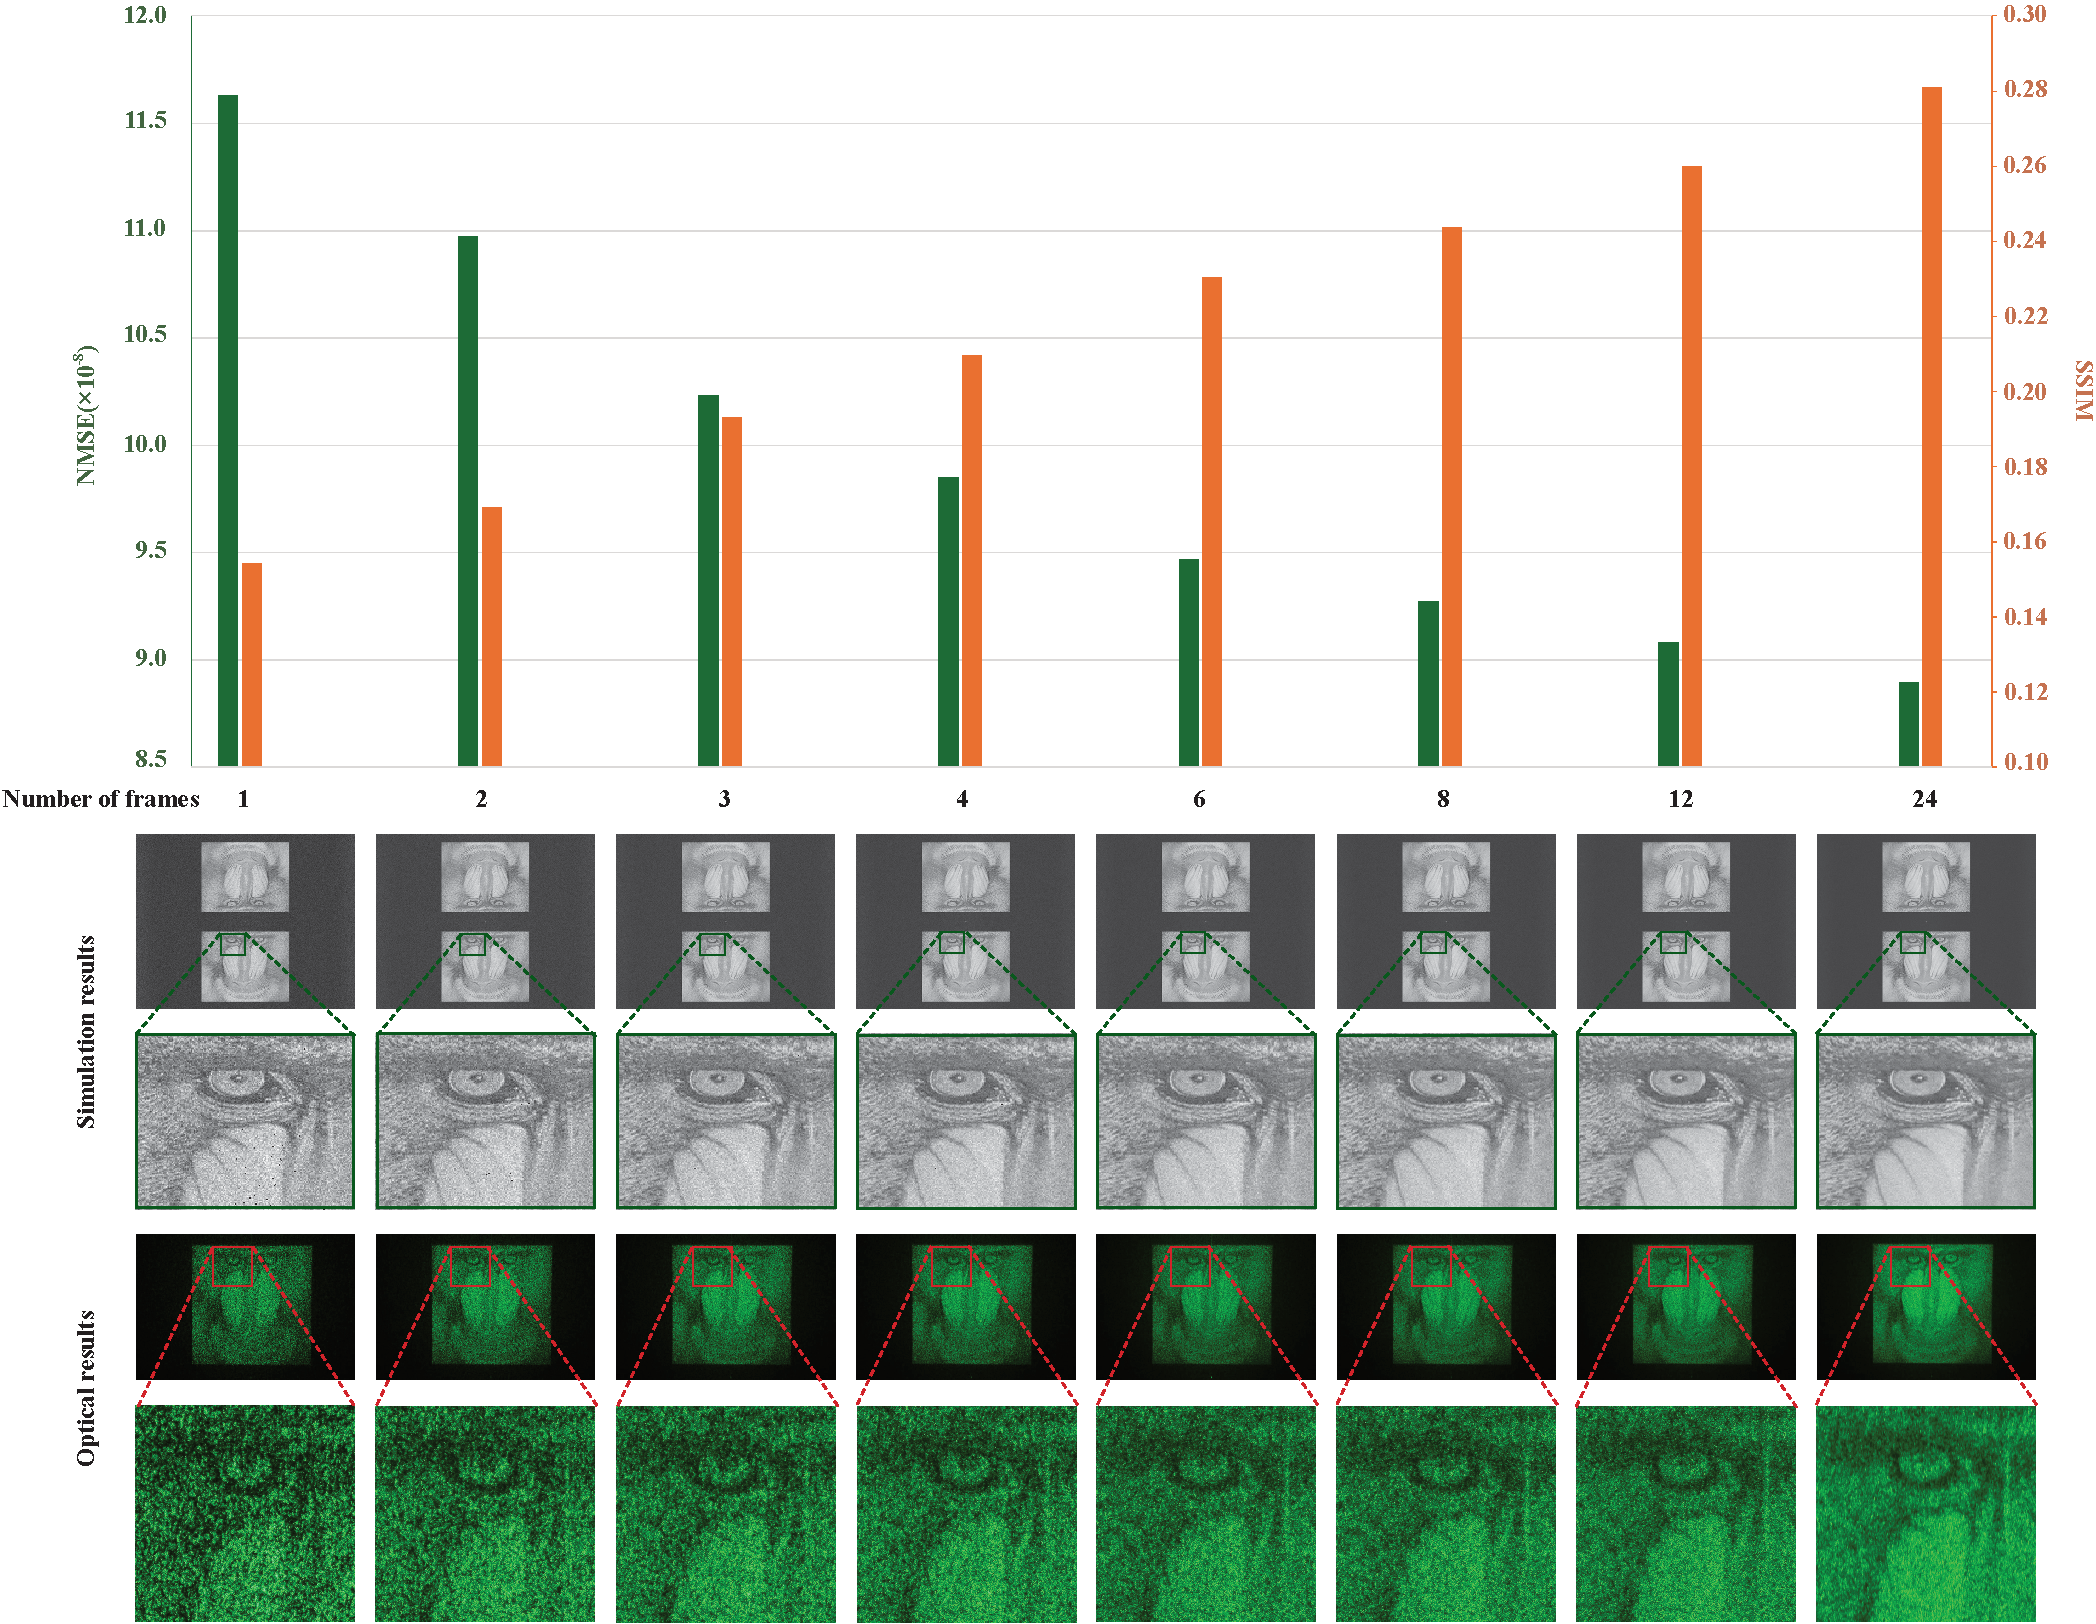
\includegraphics[width=1.0\textwidth]{recon_quality_vs_num_frames.pdf}
		\caption{Simulation and optical reconstruction results for different number of frames}
		\label{fig:recon_quality_vs_num_frames}
	\end{figure}

	The results in \cref{fig:recon_quality_vs_num_frames} further compares the final results for different number of frames. The histogram in \cref{fig:recon_quality_vs_num_frames} shows that, as the number of frames increases, the NMSE between the average reconstructions $\textbf{R}_{avg}$ and the target image $\textbf{T}$ decreases and the structural similarity index (SSIM)\cite{Wang2004_SSIM} increases, showing a trend of better reconstruction quality with higher number of frames. Such a trend is expected as more frames provide higher information capacity, which agrees with the information capacity research in \cref{chapter:information capacity} where holograms with higher bit depth were found to achieve better reconstruction quality. The trend is also shown visually via the simulation results and their detail enlargements. The corresponding multi-frame holograms are then loaded onto the SLM, and the reconstructed field is captured using a camera of model Canon EOS 1000D. Only the bottom halves of the reconstructed field were captured as the symmetrical conjugates were unwanted feature of far field projections from binary-phase SLM's. The raw data including multi-frame binary-phase holograms, simulated reconstruction and optical results captured are accessible in the database \cite{research_data_MFHO2024}.

	\begin{figure}[H]
		\centering
		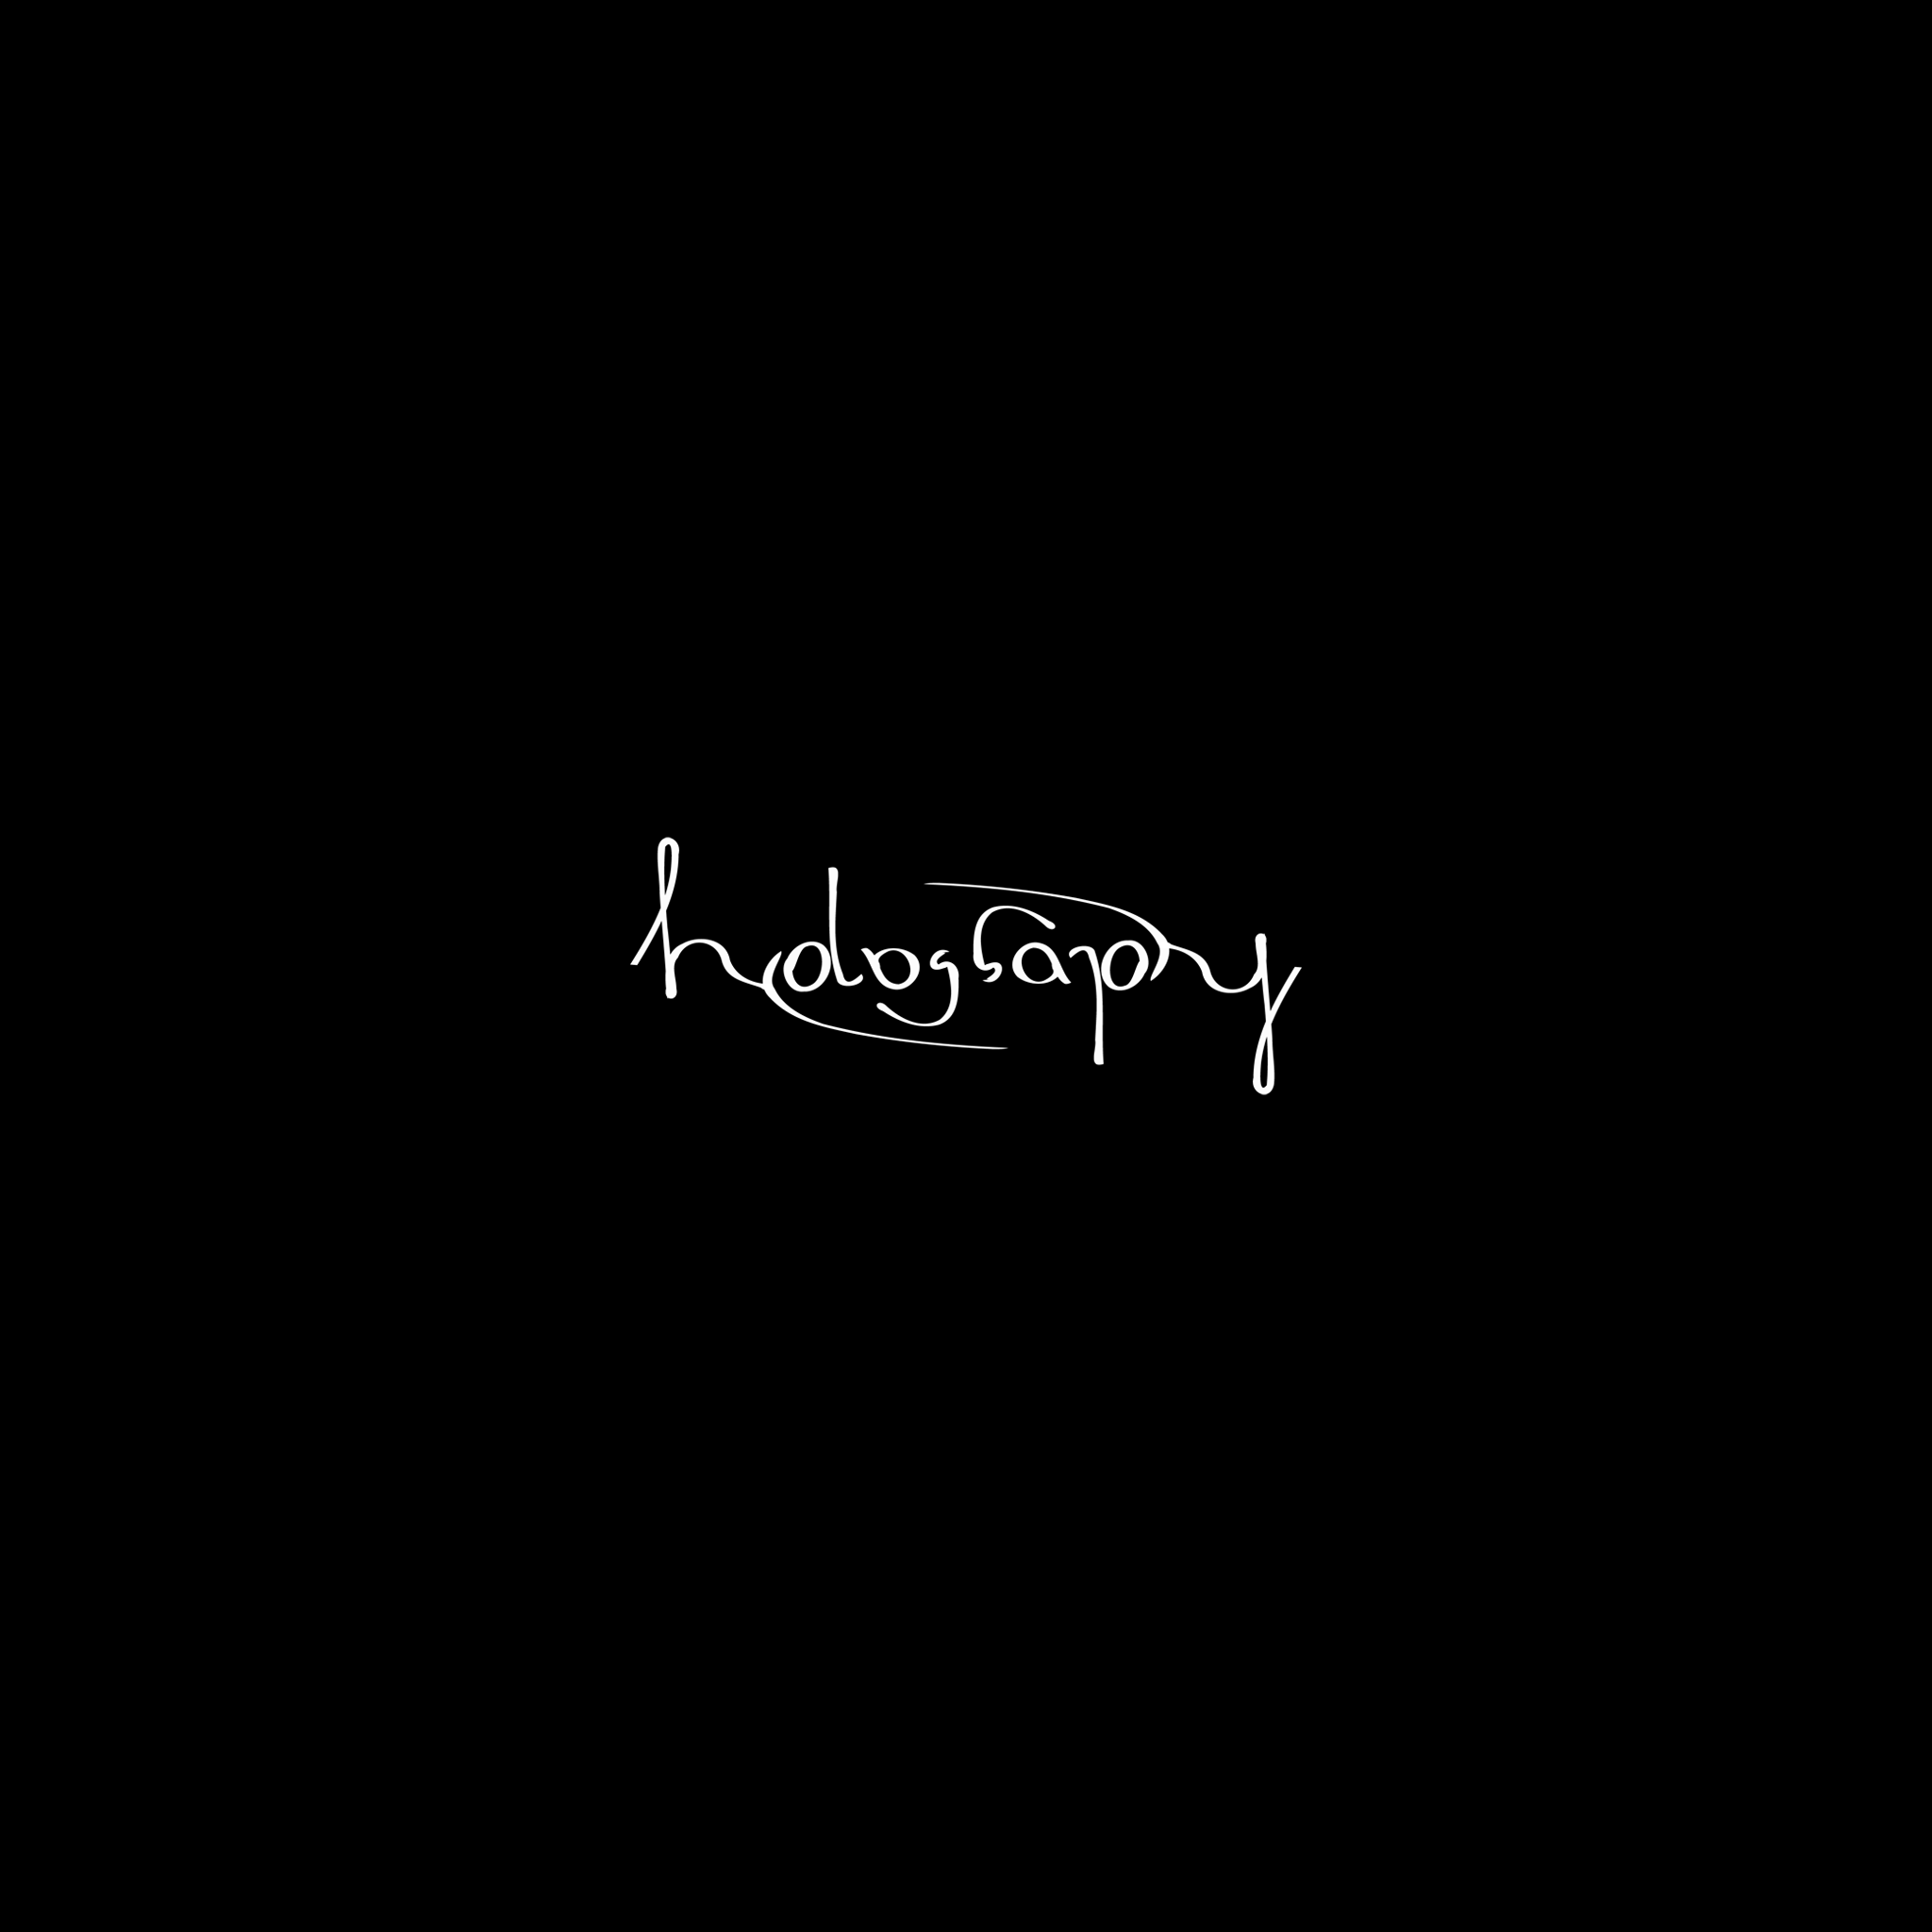
\includegraphics[width=0.5\linewidth]{holography_ambigram_smaller.png}
		\caption{Sample target image - `holography' ambigram}
		\label{fig:holography_ambigram_smaller}
	\end{figure}

	Then another target image was tested, which is the holography ambigram shown  as shown in \cref{fig:holography_ambigram_smaller}.\footnote{Adapted, with colours reversed, from  \emph{holography} - Benjamin Wetherfield, 2022.} The term ambigram is used to refer to (often typographical) designs that are invariant under a reflection, rotation or other symmetry. The `holography' design contains 180-degree rotational symmetry, which makes it especially well suited to binary Fourier-holographic projection, where this symmetry is unavoidable. Multi-frame holograms were then generated using the proposed MFHBO method and the existing OSPR and AD-OSPR methods, for the same number of frames $n=24$. And the optical results are shown in \cref{fig:recon_quality_vs_OSPR_ADOSPR}.

	\begin{figure}[H]
		\centering
		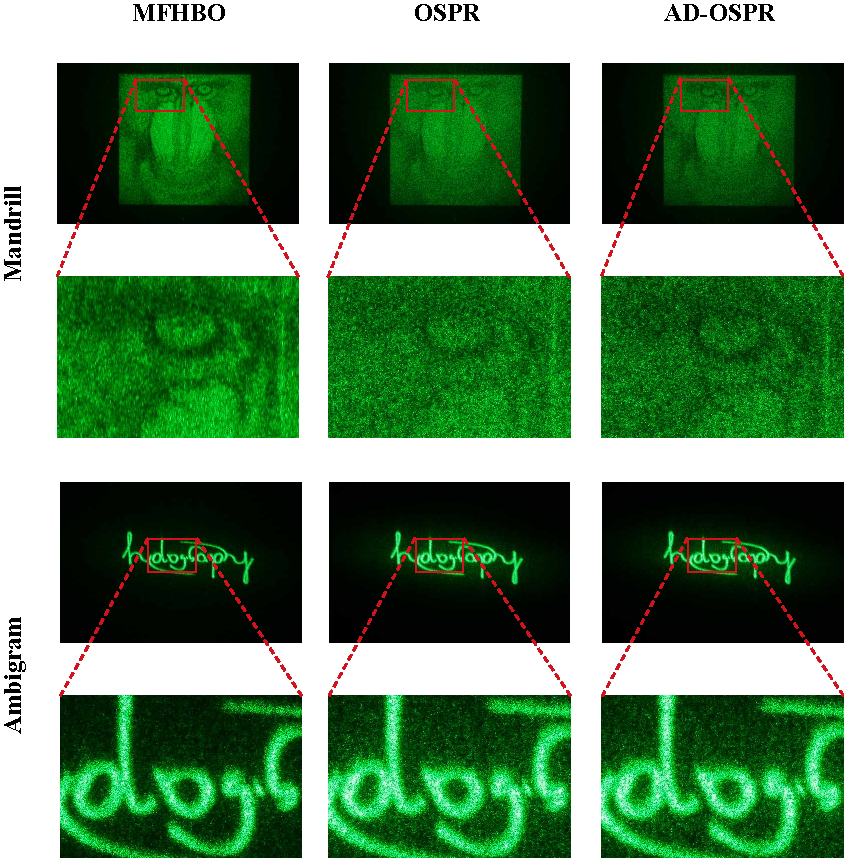
\includegraphics[width=1.0\textwidth]{recon_quality_vs_OSPR_ADOSPR.pdf}
		\caption{Optical results comparison of the proposed MFHBO method against the existing OSPR and AD-OSPR methods}
		\label{fig:recon_quality_vs_OSPR_ADOSPR}
	\end{figure}

	As shown in \cref{fig:recon_quality_vs_OSPR_ADOSPR}, for the Mandrill target image, it can be seen that the proposed MFHBO method achieved a much better optical reconstruction quality than the existing OSPR and AD-OSPR methods, with clearer details and better contrasts; for the `holography' ambigram target image, the proposed MFHBO method is shown to have a much lower background noise around the centre, than the existing OSPR and AD-OSPR methods. The intended black regions are represented much more cleanly, with an elimination of speckle-like artefacts in the zero-valued space around the lettering, and an overall increase in discernible contrast.

	\begin{table}[H]
	\centering
	\begin{tabular}{|c|c|c|c|c|}
	\hline
	\textbf{Image}              & \textbf{Metric}    & \textbf{MFHBO}  & \textbf{OSPR}  & \textbf{AD-OSPR} \\ \hline
	\multirow{2}{*}{Mandrill}   & NMSE ($\times 10^{-4}$) & 0.84      & 1.00           & 1.12             \\ \cline{2-5}
								& SSIM               & 0.124          & 0.076          & 0.078            \\ \hline
	\multirow{2}{*}{Ambigram}   & NMSE ($\times 10^{-5}$) & 2.29      & 3.31           & 3.23             \\ \cline{2-5}
								& SSIM               & 0.795          & 0.826          & 0.827            \\ \hline
	\end{tabular}
	\caption{Quantitative analysis of the optical results in \cref{fig:recon_quality_vs_OSPR_ADOSPR}}
	\label{tab:quantitative_vs_OSPR_ADOSPR}
	\end{table}

	A quantitative analysis was then conducted on the optical results in \cref{fig:recon_quality_vs_OSPR_ADOSPR}, the NMSE and SSIM between the captured reconstructions and there corresponding targets are computed and listed in \cref{tab:quantitative_vs_OSPR_ADOSPR}. The NMSE results of the proposed MFHBO method are lower than those of the existing OSPR and AD-OSPR methods, with a 25\% reduction on average among both target images. On the other hand, the SSIM results have shown a 62\% increase using MFHBO than OSPR and AD-OSPR for the mandrill target image, but a slight decrease of 3.7\% for the `holography' ambigram target image, which is negligible as it is less than 5\% and the SSIM metric is not originally designed for binary-valued non-greyscale images.

\subsubsection{3D Holography}

	\begin{figure}[H]
		\centering
		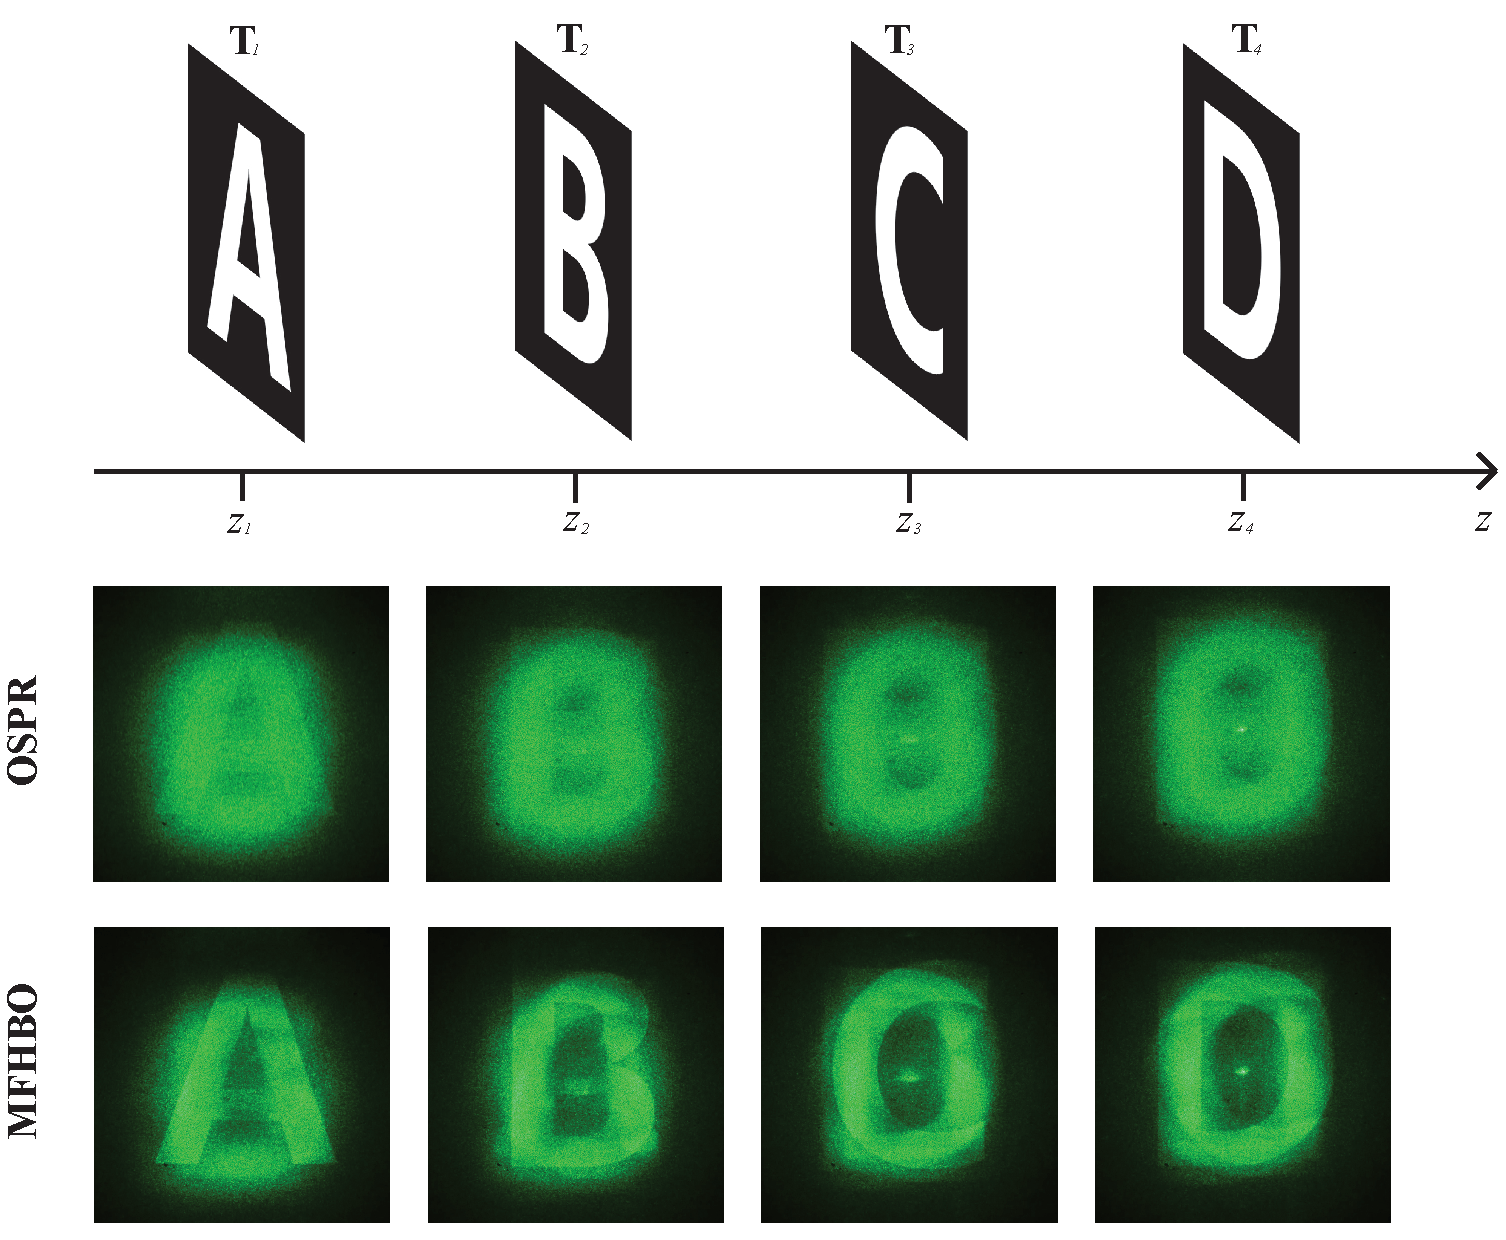
\includegraphics[width=1.0\textwidth]{MFHO_OSPR_ABCD.pdf}
		\caption{4-slice target and according reconstruction results}
		\label{fig:MFHO_OSPR_ABCD}
	\end{figure}

	The proposed MFHBO method was extended to multi-slice targets, by computing the loss between all 4 slices of reconstructions and target images (the Sum-of-Loss method in \cite{Sha2023}). An example 4-slice target made from letters `A, B, C, D' is shown in \cref{fig:MFHO_OSPR_ABCD}. The $z$ values, corresponded to the $z$ variable in \cref{eq:fresnel-diffraction}, were chosen to be $1.1m, 1.9m, 3.5m, 7.7m$ for the 4 slices respectively (as there's no correlation between each slice, larger separation was chosen for fewer cross-talk across different planes). It can be seen that the proposed MFHBO method has produced sharper edges in reconstruction than the existing OSPR method. (The AD-OSPR method was not attempted here as its application to multi-slice targets was not defined).

	\begin{table}[H]
	\centering
	\begin{tabular}{|c|c|c|c|c|c|c|}
	\hline
	\textbf{Method} & \textbf{Metric} & \textbf{Slice 1} & \textbf{Slice 2} & \textbf{Slice 3} & \textbf{Slice 4} & \textbf{Average} \\ \hline
	\multirow{2}{*}{OSPR} & NMSE($\times 10^{-4}$) & 4.980 & 4.484 & 5.644 & 4.846 & 4.988 \\ \cline{2-7}
						  & SSIM                   & 0.072 & 0.061 & 0.048 & 0.060 & 0.060 \\ \hline
	\multirow{2}{*}{MFHO} & NMSE($\times 10^{-4}$) & 4.484 & 4.230 & 4.990 & 4.289 & 4.498 \\ \cline{2-7}
						  & SSIM                   & 0.063 & 0.067 & 0.058 & 0.072 & 0.065 \\ \hline
	\end{tabular}
	\caption{Quantitative analysis of the optical results in \cref{fig:MFHO_OSPR_ABCD}}
	\label{tab:quant_MFHO_OSPR_ABCD}
	\end{table}

	Then a quantitative analysis was carried out, with NMSE and SSIM values measured and shown in \cref{tab:quant_MFHO_OSPR_ABCD}. The proposed MFHBO method has shown a 10\% reduction in NMSE and a 8\% improvement in SSIM on average than the existing OSPR method, demonstrating the effectiveness of the proposed method.


	\begin{figure}[H]
		\centering
		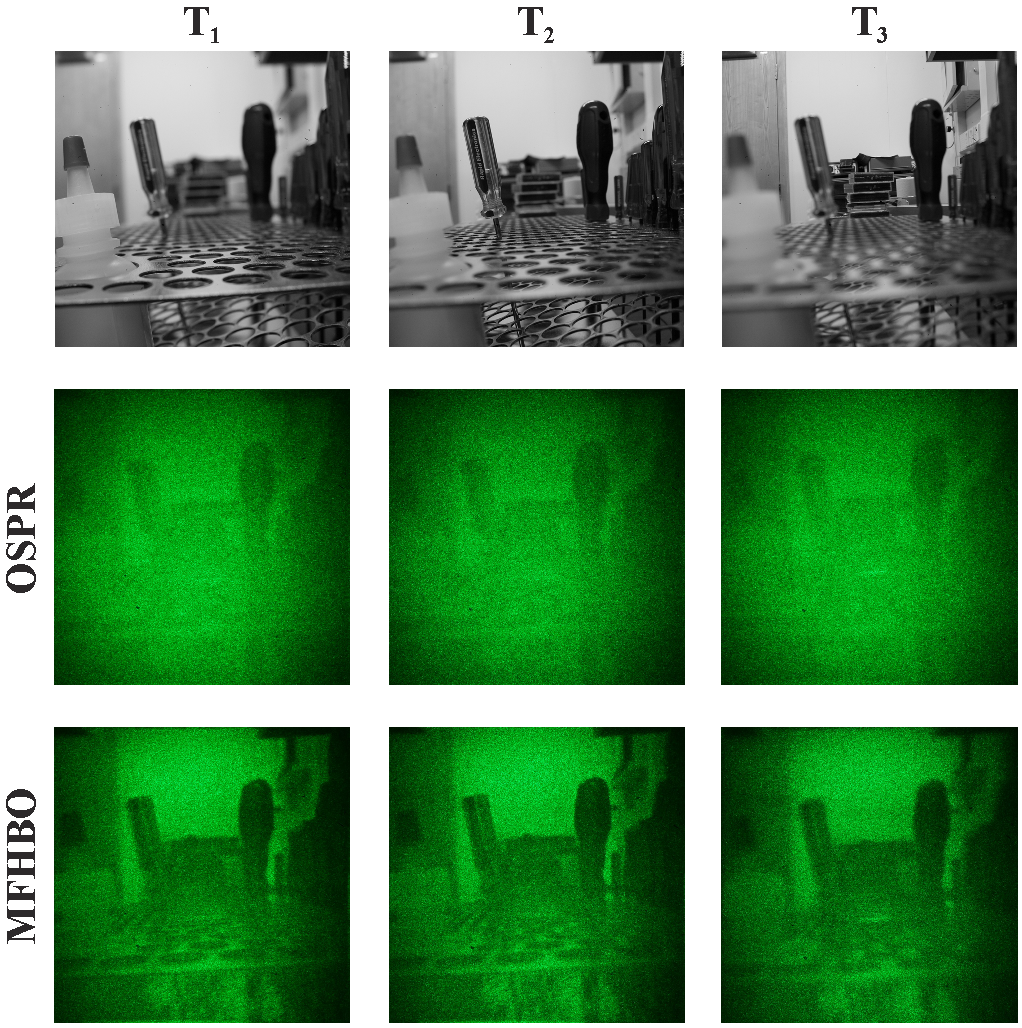
\includegraphics[width=1.0\textwidth]{MFHO_OSPR_Pen_holder.pdf}
		\caption{Real-life captured image as target field and their reconstruction results}
		\label{fig:MFHO_OSPR_Pen_holder}
	\end{figure}

	Lastly, a set of real-life scene was captured in the lab using near, middle and far focus, as shown in $\textbf{T}_1, \textbf{T}_2, \textbf{T}_3$ in \cref{fig:MFHO_OSPR_Pen_holder} respectively. The $z$ values were set to $1.1m, 1.2m, 1.3 m$ for hologram generation, and the reconstruction results of the existing OSPR and the proposed MFHBO methods are compared in \cref{fig:MFHO_OSPR_Pen_holder}. The proposed MFHBO method is shown to have achieved better reconstruction quality than the existing OSPR method.

	\begin{table}[H]
	\centering
	\begin{tabular}{|c|c|c|c|c|c|}
	\hline
	\textbf{Method} & \textbf{Metric} & \textbf{Slice 1} & \textbf{Slice 2} & \textbf{Slice 3} & \textbf{Average} \\ \hline
	\multirow{2}{*}{OSPR} & NMSE($\times 10^{-6}$) & 3.70 & 3.69 & 3.47 & 3.62 \\ \cline{2-6}
						  & SSIM                   & 0.37 & 0.28 & 0.34 & 0.33 \\ \hline
	\multirow{2}{*}{MFHO} & NMSE($\times 10^{-6}$) & 3.20 & 2.78 & 3.06 & 3.01 \\ \cline{2-6}
						  & SSIM                   & 0.42 & 0.32 & 0.32 & 0.35 \\ \hline
	\end{tabular}
	\caption{Quantitative analysis of the optical results in \cref{fig:MFHO_OSPR_Pen_holder}}
	\label{tab:quant_MFHO_Pen_holder}
	\end{table}

	A quantitative analysis was conducted again, with NMSE and SSIM values measured and listed in \cref{tab:quant_MFHO_Pen_holder}. The proposed MFHBO method has shown a 17\% reduction in NMSE and a 7\% improvement in SSIM on average than the existing OSPR method, proving the effectiveness of the proposed method.


\section{Summary}
	This chapter proposed the MFHBO method to generate multi-frame binary-phase holograms to be displayed on a high refresh rate binary-phase SLM. The proposed MFHBO method was shown to achieve much better reconstruction quality and higher contrast than the existing multi-frame binary-phase hologram generation methods OSPR \cite{Cable2004} and AD-OSPR \cite{Kaczorowski2016} on the holographic projector with a binary-phase SLM, for all the single-slice far-field targets and the multi-slice near-field targets tested. Although the proposed MFHBO method is slower than the existing OSPR and AD-OSPR methods, its much better reconstruction quality makes it suitable for pre-computed high-quality hologram applications. Its strong advantage for high contrast target such as the `holography' ambigram in \cref{fig:holography_ambigram_smaller}, with much suppressed noise in the background, makes it well-suited for photo-lithography applications. The proposed method can also be adapted for multi-level SLM's by simply removing the quantisation step in \cref{fig:MFHO_flowchart}. This could be the case for applications such as photo-lithography, where the time response of the system is much longer than it is for human vision, and the high refresh rates of the SLM are not necessary.


	% The results are compared to One-Step Phase-Retrieval and Adaptive One-Step Phase-Retrieval in simulation and experimentally, proving the superiority of the proposed approach. This technique can be easily extended to other spatial modulation methods.